\chapter{Metodologia}
\section{Visão Global}
Definiu-se, inicialmente, como a equipe irá trabalhar para construir o robô proposto. Estabeleceu-se as ferramentas, divisão de trabalho, controle de custos, organização de diretórios do projeto, próximas atividades, entre outros.

\subsection{Equipe}
A equipe do projeto foi dividida em duas grande áreas de trabalho: Estrutural e Lógica, como apresentado na figura abaixo.

\begin{figure}[h]
    \centering
    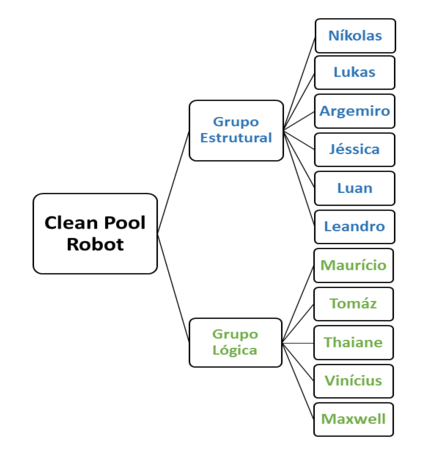
\includegraphics[width=0.8\textwidth]{figures/equipe.png}
    \caption{Divisão das equipes para desenvolvimento do projeto.}
    \label{fig:schema-way-robot}
  \end{figure}
  
\par A primeira equipe, Estrutural, está encarregada de desenvolver a parte eletromecânica do robô. Este grupo foi composto pelos estudantes das engenharias Aeroespacial, Automotiva e de Energia. 
\par O segundo grupo, Lógica, é responsável pela parte de eletrônica e software embarcados no produto, sendo composto pelos estudantes das respectivas engenharias.

\subsection{Forma de Trabalho}
A comunicação  do grupo é realizada por meio de ferramentas \textit{online}, tais como, \textit{Google Drive}, \textit{Trello}, \textit{WhatsApp}, \textit{Github} e \textit{Hangout}, além de reuniões semanais na Faculdade Gama, vislumbrando o gerenciamento ativo das propostas.
\par As ferramentas citadas auxiliam a equipe no compartilhamento e criação de documentos e arquivos que facilitam o projeto e a troca de informações, orientações e demandas de forma mais ágil e imediata entre os integrantes da equipe.

\subsection{Macro Planejamento}
O projeto terá três pontos de controle, onde serão apresentados o que foi produzido até o momento para um grupo de professores que auxiliarão a direcionar a execução do projeto. Planejou-se entregar em cada ponto de controle o descrito abaixo:

% Please add the following required packages to your document preamble:
% \usepackage{booktabs}
\begin{table}[h]
\centering
\caption{My caption}
\label{my-label}
\begin{tabular}{@{}|l|l|l|l|l@{}}
\cmidrule(r){1-4}
\textbf{\begin{tabular}[c]{@{}l@{}}Ponto de \\ Controle\end{tabular}} & \textbf{\begin{tabular}[c]{@{}l@{}}Data de \\ Entrega\end{tabular}} & \textbf{Entregável}                                                                                                                                            & \textit{\textbf{Status}} &  \\ \cmidrule(r){1-4}
1º                                                                    & 15/04/16                                                            & \begin{tabular}[c]{@{}l@{}}Escopo, pesquisa de concorrentes, croquis iniciais,\\  esquemáticos e solução proposta\end{tabular}                                 & Realizado                &  \\ \cmidrule(r){1-4}
2º                                                                    & 27/05/16                                                            & \begin{tabular}[c]{@{}l@{}}Teste dos módulos do Clean Pool (movimentação, \\ filtragem, sensores, vedação do circuito, percurso, \\ entre outros)\end{tabular} & Previsto                 &  \\ \cmidrule(r){1-4}
3º                                                                    & 01/07/16                                                            & Clean Pool Robot e documentação do projeto                                                                                                                     & Previsto                 &  \\ \cmidrule(r){1-4}
\end{tabular}
\end{table}
\FloatBarrier

\subsection{Controle de Custos}
A equipe do projeto considerou necessário o controle de custos financeiros com compra de material para construção do \textit{Clean Pool Robot}. Sendo assim, foi elaborado uma planilha para auxiliar nesse controle.

\par O custo orçado total com material é de R\$ 1254,20. Considerou-se 10\% a mais com materiais não previstos. Com isso, o custo orçado total é de R\$ 1379,62, o que resulta em R\$ 125,42 por integrante.

\begin{figure}[h]
    \centering
    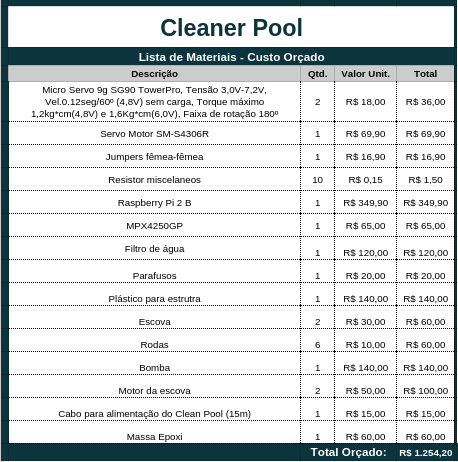
\includegraphics[width=\textwidth]{figures/custos.png}
    \caption{Parte da tabela de controle de custos.}
    \label{fig:schema-way-robot}
  \end{figure}
\FloatBarrier
\par Para controle do custo real, serão registrados as compras realizadas para construção do \textit{Clean Pool Robot}, bem como o valor e o nome do integrante que forneceu o dinheiro. Com esse controle será possível reembolsar os integrantes que tiveram prejuízo.


  